\section{Sizing under Real-World Energy Conditions} \label{sec:c4_demo}

In this section, we model an IPS with a PV energy harvester to explore the energy storage sizing effect in real-world energy conditions, and demonstrate use of the proposed sizing approach. 

\begin{figure}
    \centering
    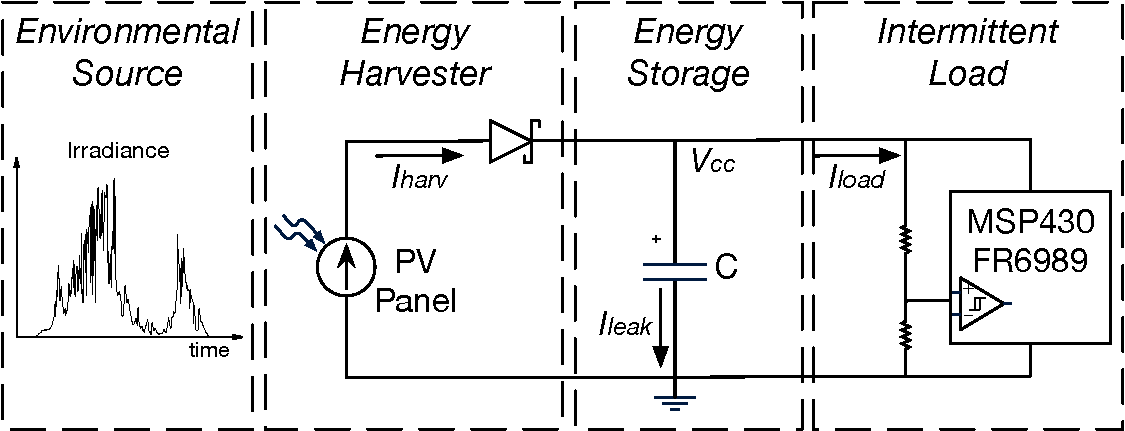
\includegraphics[width=\columnwidth]{ch4_sizingapproach/figures/solarmodel4}
    \caption{System model of a PV-based IPS.}
    \label{fig:Model}
\end{figure}

\subsection{Simulation Configuration}

We integrate the validated reactive IPS model into a system model with a PV energy-harvesting supply as shown in \fref{fig:Model}. 
The energy storage model and the intermittent load model are as presented in \sref{sec:c3_exploration}. 

We use a converter-less supply circuit where only a Schottky diode is connected to the energy harvester output in order to prevent current backflow. 
The energy source conditions are imported from NREL outdoor solar irradiance data~\cite{stoffel1981nrel} and EnHANTs indoor irradiance data~\cite{6244798}. 
Four sets of light conditions are used to encompass different energy environments. 
To convert irradiance into harvested power, we adopt a PV cell model~\cite{en9050326} which uses the parameters available in common datasheets, so it can easily be reconfigured to suit various devices. 
The output current \nm{I}{o} of the PV cell model can then be described as:
\begin{equation} \label{eq:pvcell}
    \nmm{I}{o} = \frac{G}{\nmm{G}{ref}} \nmm{I}{sc} (1 - (1 - \frac{\nmm{I}{mpp}}{\nmm{I}{sc}}) ^ {\frac{\nmm{V}{o}-\nmm{V}{oc}}{\nmm{V}{mpp} - \nmm{V}{oc}}})
\end{equation}
where \nm{V}{o} is the output voltage of the PV cell, $G$ is the ambient irradiance, \nm{G}{ref} is the reference irradiance (normally \SI{1000}{\watt\per\square\centi\meter}), and \nm{I}{sc}, \nm{V}{oc}, \nm{I}{mpp}, \nm{V}{mpp} are respectively short-circuit current, open-circuit voltage, and the current and voltage at maximum power point (MPP) given the reference irradiance. 
\nm{V}{o} and $G$ are dynamic at run time, while other parameters in this model are constant. 
We refer to Panasonic Amorton glass type solar cells~\cite{solarcell} for PV cell properties as shown in \tref{tab:pvcell}. 
We set four cells in series (with \nm{V}{oc} = 3.56V) to match the operating voltage of the MCU (maximum 3.6V), and model energy harvester sizing by scaling the cell area. 


% A PV panel is an array of PV cells, which amplifies voltage and current output by connecting PV cells in series or parallel. In a PV panel, the open-circuit voltage is proportional to the number of cells in series, and the short-circuit current is proportional to the area of each cell and the number of cells in parallel. 

\begin{table}
    \renewcommand{\arraystretch}{1.2}
    \centering
    % \caption{PV Cell Properties under AM1.5 1000W/m$^2$ Light Conditions.}
    \caption{PV cell properties under a \SI{1000}{\watt\per\square\centi\meter}, AM-1.5 light source}
    \label{tab:pvcell}
    \begin{tabular}{|c|c|}
    \hline
    \textbf{Parameter} & \textbf{Value}\\
    \hline
    Open-Circuit Voltage & \SI{0.89}{\volt}/cell\\
    Short-Circuit Current & \SI{14.8}{\milli\ampere\per\square\centi\meter}\\
    Maximum Power Voltage & \SI{0.65}{\volt}/cell\\ 
    Maximum Power Current & \SI{12.1}{\milli\ampere\per\square\centi\meter}\\
    \hline
    \end{tabular}
\end{table}

Our simulation tool can perform two simulation processes: (a) sort and process the time distribution of environmental conditions, and (b) simulate system state chronologically with a fine-grained time step. 
Process (a) reduces simulation time significantly, e.g. from hours to seconds, but ignores the restore operation after a brownout reset, hence overestimating forward progress, and it overestimates more with smaller capacitance and lower supply current. 
In the following results, \fref{fig:harvstor} comes from Process (a) for fast exploration, and \fref{fig:interruption} and \fref{fig:tradeoff} come from Process (b) for accurate records of interruption periods. 

\subsection{Exploration with Real-World Energy Source Conditions} \label{subsec:harvstor}

% Goal: 
% 1. to show that this model can help designers to find a suitable size of EH to achieve their desired performance;
% 2. to show that sizing energy storage would have different degrees of impact on real deployment depending on the specific energy conditions;
% 3. demonstrate sizing approach. 

In real-world deployments, ambient energy source conditions are dependent on time and location. 
The energy harvester and storage need to be sized to achieve the desired forward progress across the range of expected conditions. 

\subsubsection{Sizing the Energy Harvester}

For the purposes of this exploration, three levels of baseline mean forward progress (\nm{\alpha}{exe}) are set as 0.1, 0.2, and 0.3. 
We use the system model to find the PV panel area that achieves the expected forward progress under the different energy source conditions with minimum energy storage. 
We scale the PV panel area to find that which achieves each baseline \nm{\alpha}{exe}. 
As shown in \fref{fig:harvstor}, the energy harvester sizes that achieve the desired \nm{\alpha}{exe} may span orders of magnitude given different energy source conditions from \SI{}{\square\milli\meter} for outdoor sources ((c) and (d)) to \SI{}{\square\centi\meter} for indoor sources ((a) and (b)).  

\subsubsection{Sizing the Energy Storage}

Having obtained the energy harvester sizes for the baseline forward progress, we then use the modelling approach to size energy storage.
% A table lists the PV panel area to achieve the target \nm{\alpha}{exe} with minimum energy storage capacitance, the optimal capacitance with the forward progress improvement, and the alternative (decreased) PV panel area with the optimal capacitance. 
We analyse the sizing effect of energy storage on forward progress given real-world energy conditions. \fref{fig:harvstor} shows a 7.8-43.3\% improvement in forward progress by sizing energy storage under the given real-world energy conditions and baseline energy harvester sizes. 
It can also be inferred that optimising energy storage can either improve forward progress for a given energy harvester size, or reduce the energy harvester size that achieves the target forward progress. 
Given higher-power energy sources (e.g. Denver 2018 and Hawaii 2018 outdoor solar), increasing the harvester size efficiently improves forward progress with minor dimensional overheads, e.g. tens of \SI{}{\square\milli\meter}; however, given lower-power sources (e.g. EnHANTs Setup~A and Setup~D indoor light), optimising energy storage capacitance can save tens of \SI{}{\square\centi\meter} of PV panel area to achieve the same forward progress.

Also, the progress improvement by sizing energy storage varies accordingly with energy source conditions. 
As mentioned in \cref{chapter:sizingeffect}, this improvement stems from the reduction of restore and save overheads when the supply current is low and the device work in the \textit{Intermittent} mode. 
Thus, the results of EnHANTs Setup~A and Setup~D show a higher progress improvement from sizing energy storage than those of Denver 2018 and Hawaii 2018. 

\begin{figure}
    \centering
    \begin{subfigure}{0.51\columnwidth}
        \centering
        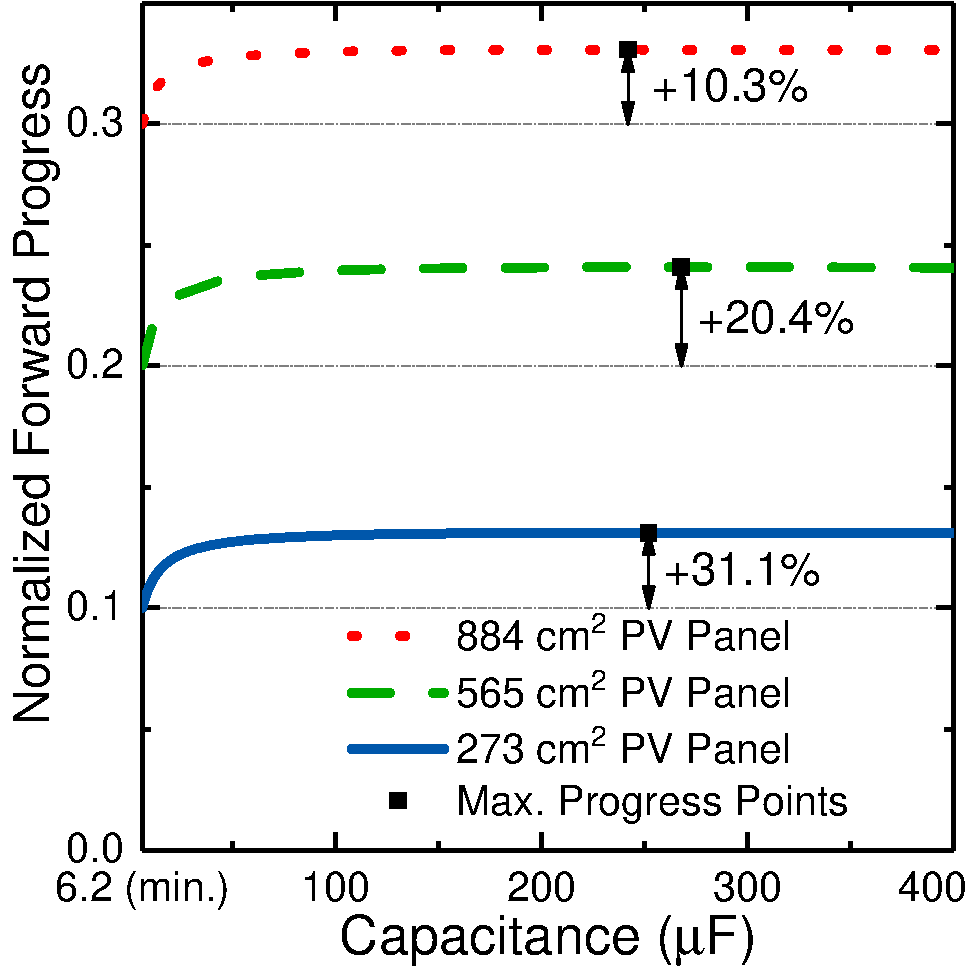
\includegraphics[width=\columnwidth]{ch4_sizingapproach/figures/HarvStorTgFig1}
        \caption{EnHANTs Setup A}
        \label{fig:harvstor1}
    \end{subfigure}
    \begin{subfigure}{0.483\columnwidth}
        \centering
        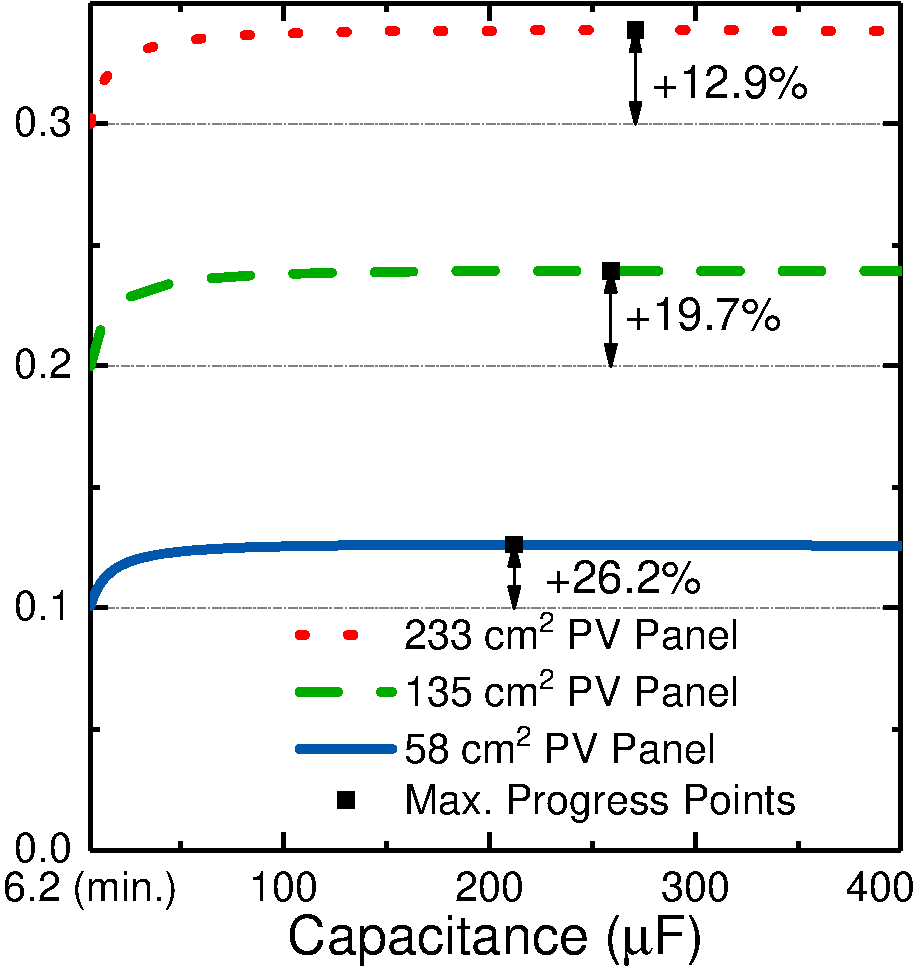
\includegraphics[width=\columnwidth]{ch4_sizingapproach/figures/HarvStorTgFig2}
        \caption{EnHANTs Setup D}
        \label{fig:harvstor2}
    \end{subfigure}
    \hfil
    \begin{subfigure}{0.51\columnwidth}
        \centering
        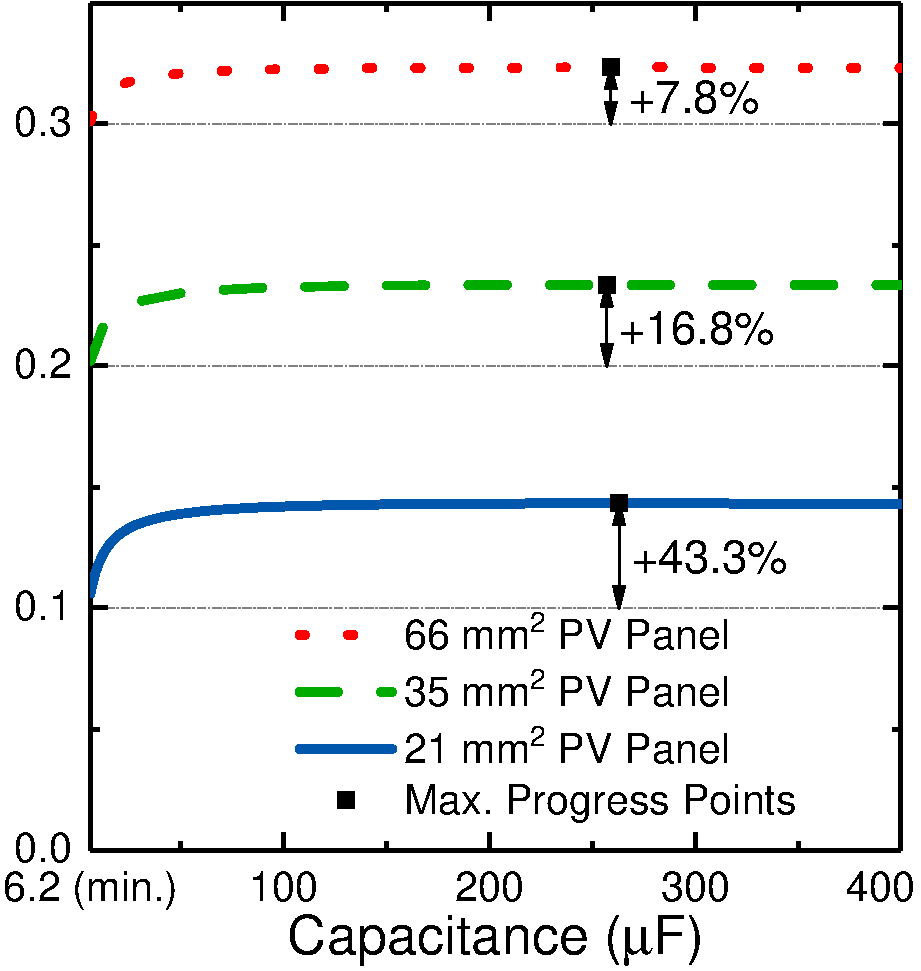
\includegraphics[width=\columnwidth]{ch4_sizingapproach/figures/HarvStorTgFig3}
        \caption{NREL Denver 2018}
        \label{fig:harvstor3}
    \end{subfigure}
    \begin{subfigure}{0.483\columnwidth}
        \centering
        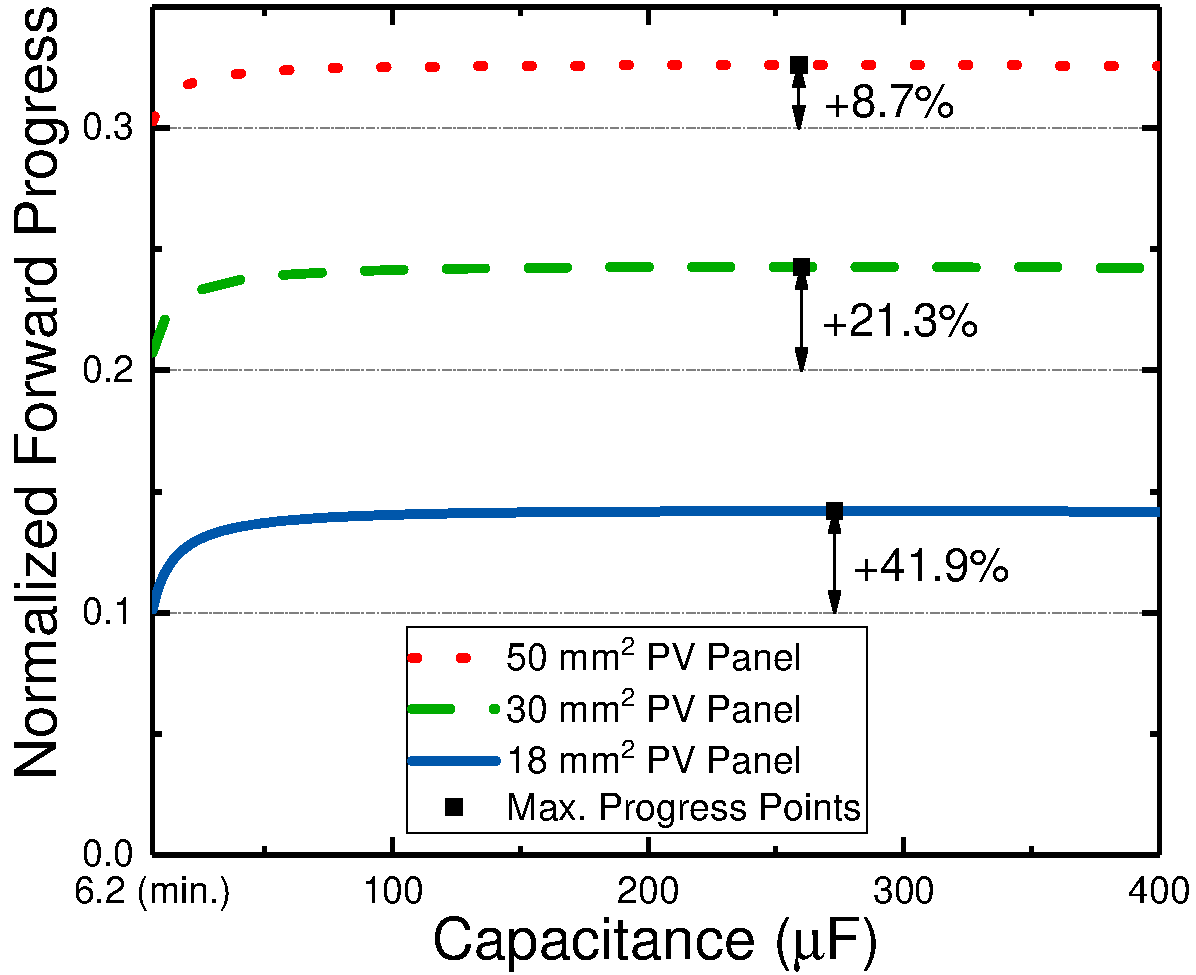
\includegraphics[width=\columnwidth]{ch4_sizingapproach/figures/HarvStorTgFig4}
        \caption{NREL Hawaii 2018}
        \label{fig:harvstor4}
    \end{subfigure}
    \caption{Improvement of average forward progress by sizing energy storage given different PV panel areas under real-world energy source conditions. The model is able to find the PV panel area required for achieving the target mean forward progress. } 
    \label{fig:harvstor}
\end{figure}

The mean forward progress given target \nm{\alpha}{exe} = 0.1 is plotted in \fref{fig:harvstorrange}, with the 60th and 90th time percentiles of forward progress. In all the  above datasets, the energy source is absent and the system is off for around \SI{55}{\percent} of time, so we plot the percentiles from the 60th. The mean progress during the energy-available periods is averaged over the energy-absent periods, so the actual mean forward progress during the energy-available periods is nearly double the annual mean. 

% Absolute improvement are different? Large variations? What other results can I add? 
% The variations of forward progress are significant due to the large variations of energy source conditions, so practical implementation should consider such variation as .
% The improved progress during the energy-available periods is averaged over the energy-absent periods, so the actual amount of improvement when energy is available is higher than the mean. (wrong statement)

\begin{figure}
    \centering
    \begin{subfigure}{0.51\columnwidth}
        \centering
        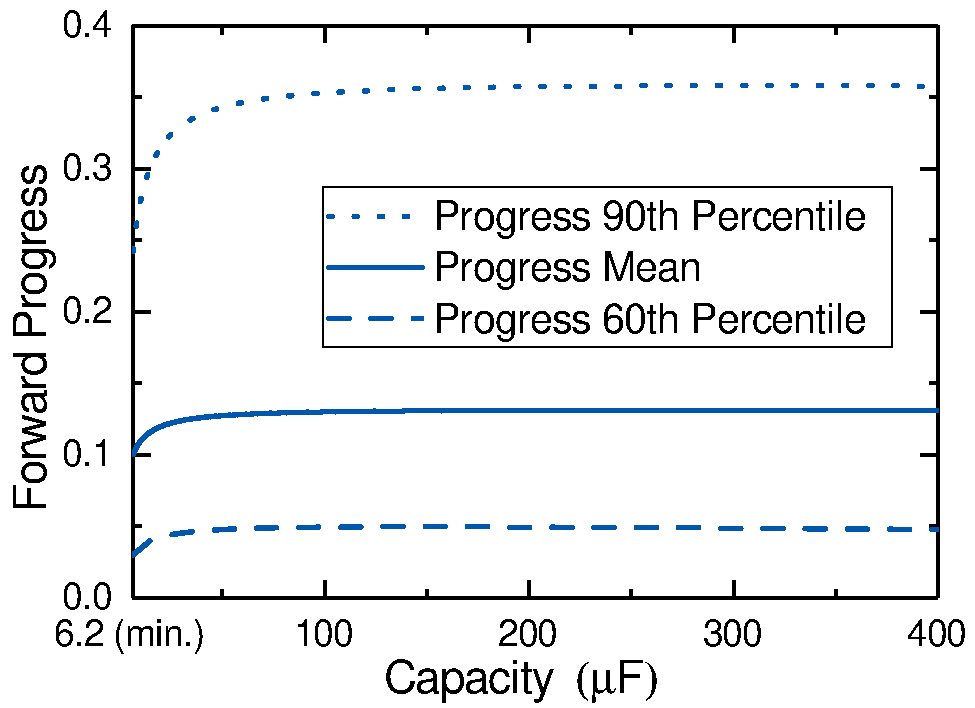
\includegraphics[width=\columnwidth]{ch4_sizingapproach/figures/HarvStorRan2Fig1}
        \caption{EnHANTs Setup A}
        \label{fig:harvstorrange1}
    \end{subfigure}
    \begin{subfigure}{0.483\columnwidth}
        \centering
        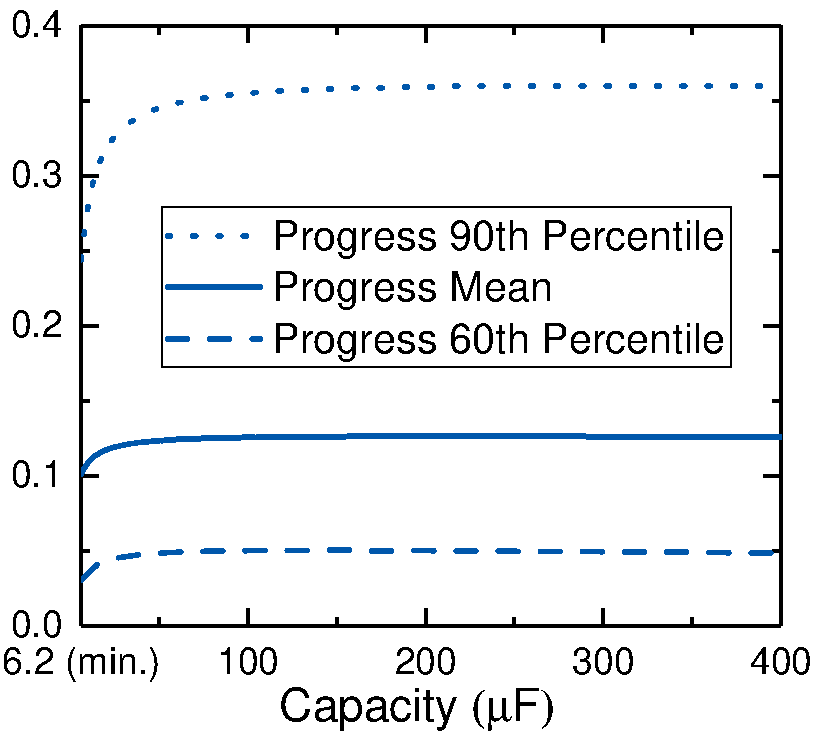
\includegraphics[width=\columnwidth]{ch4_sizingapproach/figures/HarvStorRan2Fig2}
        \caption{EnHANTs Setup D}
        \label{fig:harvstorrange2}
    \end{subfigure}
    \hfil
    \begin{subfigure}{0.51\columnwidth}
        \centering
        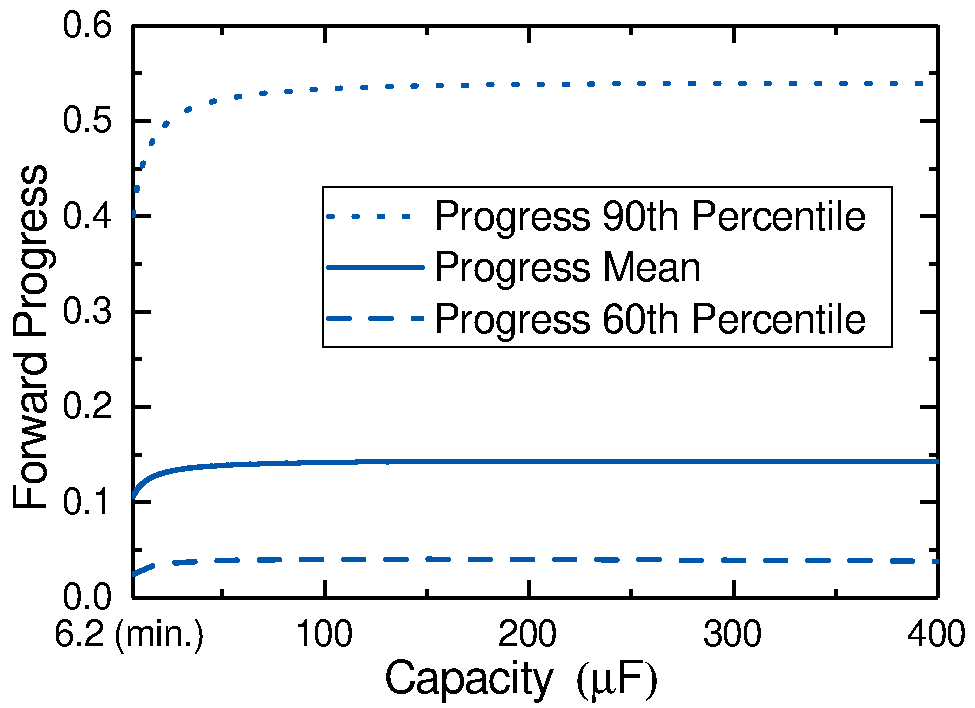
\includegraphics[width=\columnwidth]{ch4_sizingapproach/figures/HarvStorRan2Fig3}
        \caption{NREL Denver 2018}
        \label{fig:harvstorrange3}
    \end{subfigure}
    \begin{subfigure}{0.483\columnwidth}
        \centering
        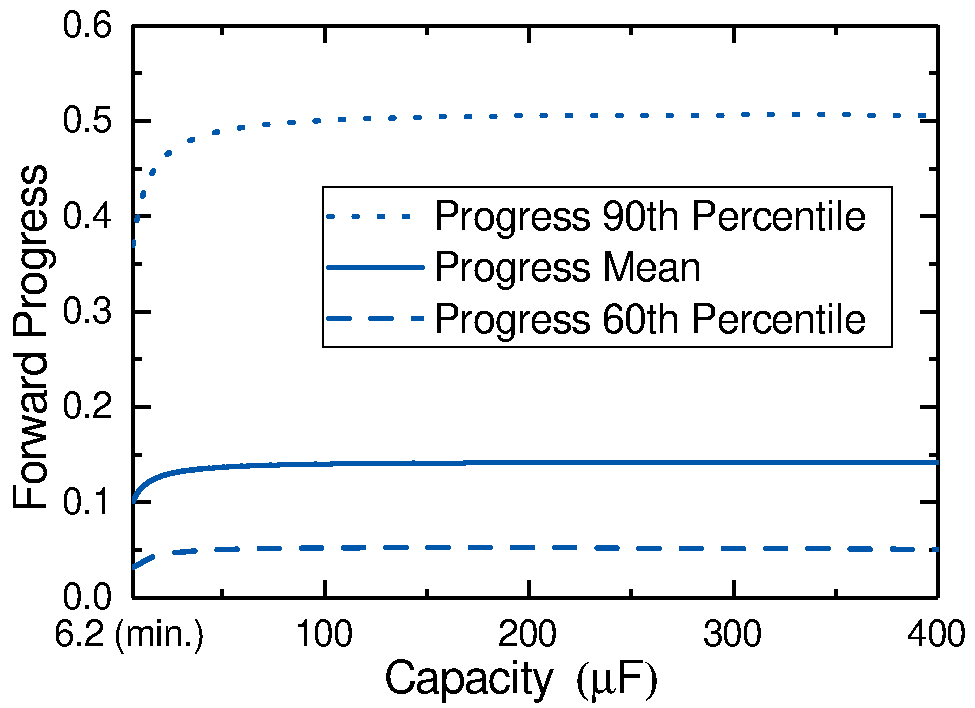
\includegraphics[width=\columnwidth]{ch4_sizingapproach/figures/HarvStorRan2Fig4}
        \caption{NREL Hawaii 2018}
        \label{fig:harvstorrange4}
    \end{subfigure}
    \caption{Time percentiles of forward progress by sizing energy storage with target \nm{\alpha}{exe} = 0.1 and the corresponding PV panel area listed in \fref{fig:harvstor}. The percentiles start from the 60th as the system is off for around \SI{55}{\percent} of time due to insufficient energy source. }
    \label{fig:harvstorrange}
\end{figure}

\subsubsection{Interruption Period} \label{subsubsec:intper}
Besides forward progress, we also explore how the capacitance can change the interruption periods. 
When interrupted by insufficient power supply, an IPS enters an interruption period where it saves its volatile state, waits for supply voltage to recover, and restores the state to resume execution, without making any forward progress. 
Applications that require frequent sensing may be negatively affected by long interruption periods. 
We measure an interruption period as \textit{the period between two successive execution periods}, e.g. a consecutive `SLR' period in \fref{fig:operatingCycle} forms an interruption period. 
We record all the interruption periods during a one-year simulation with \SIrange{10}{50}{\micro\farad} capacitors, the Denver 2018 dataset, and an \SI{80}{\square\milli\meter} PV panel. 
\fref{fig:interruption} presents the distribution of all the interruption periods. 
With increased energy storage, the interruption period is prolonged. 
For example, the 90th percentile of interruption periods increases from \SI{32.2}{\milli\second} at \SI{10}{\micro\farad} to \SI{123.4}{\milli\second} at \SI{50}{\micro\farad} at an approximate rate of \SI{23}{\milli\second} per \SI{10}{\micro\farad}. 
% The majority of the interruption periods are within \SI{200}{\milli\second}. 
Facilitated by the simulator, developers are enabled to estimate whether the distribution of interruption periods meet their application requirement. 

% Whether and how much this would affect  Time-sensitive applications may care 
% the total number of interruptions is reduced,


\begin{figure}
    \centering
    \includegraphics[width=\columnwidth]{ch4_sizingapproach/figures/IntPeriodOrdFig}
    \caption{Distribution of interruption periods. }
    \label{fig:interruption}
\end{figure}

\subsection{Trading Forward Progress, Dimensions, and Interruption Period} \label{subsec:tradeoff}

Although increasing energy storage capacitance improves forward progress, larger capacitance increases both dimensions and interruption periods. 
We evaluate the overheads of increased capacitor dimensions and interruption periods, and then trade them off against forward progress using a cost function to suggest an optimal capacitance value. 

\subsubsection{Metric of Dimensions}

The overhead of capacitor dimensions is evaluated by characteristics of off-the-shelf tantalum capacitors. 
We narrow down the range of sample capacitors within a set of characteristics: low-profile, 10V rated voltage, and surface-mount package, and select six series of capacitors\footnote{The series of capacitor considered were: AVX TAJ, AVX TACmicrochip, AVX F92, Vishay 572D, Vishay 591D, and Vishay 592D.}. 
The volume and capacitance of these devices are plotted in \fref{fig:capvol}. 
We use the regression of these data to approximate a capacitance-volume relationship.
% ~\cite{tancap1, tancap2, tancap3, tancap4, tancap5, tancap6}
% Among the common capacitor chemistries with \textmu F to mF capacitance, tantalum capacitors manifest low leakage 

\begin{figure}
    \centering
    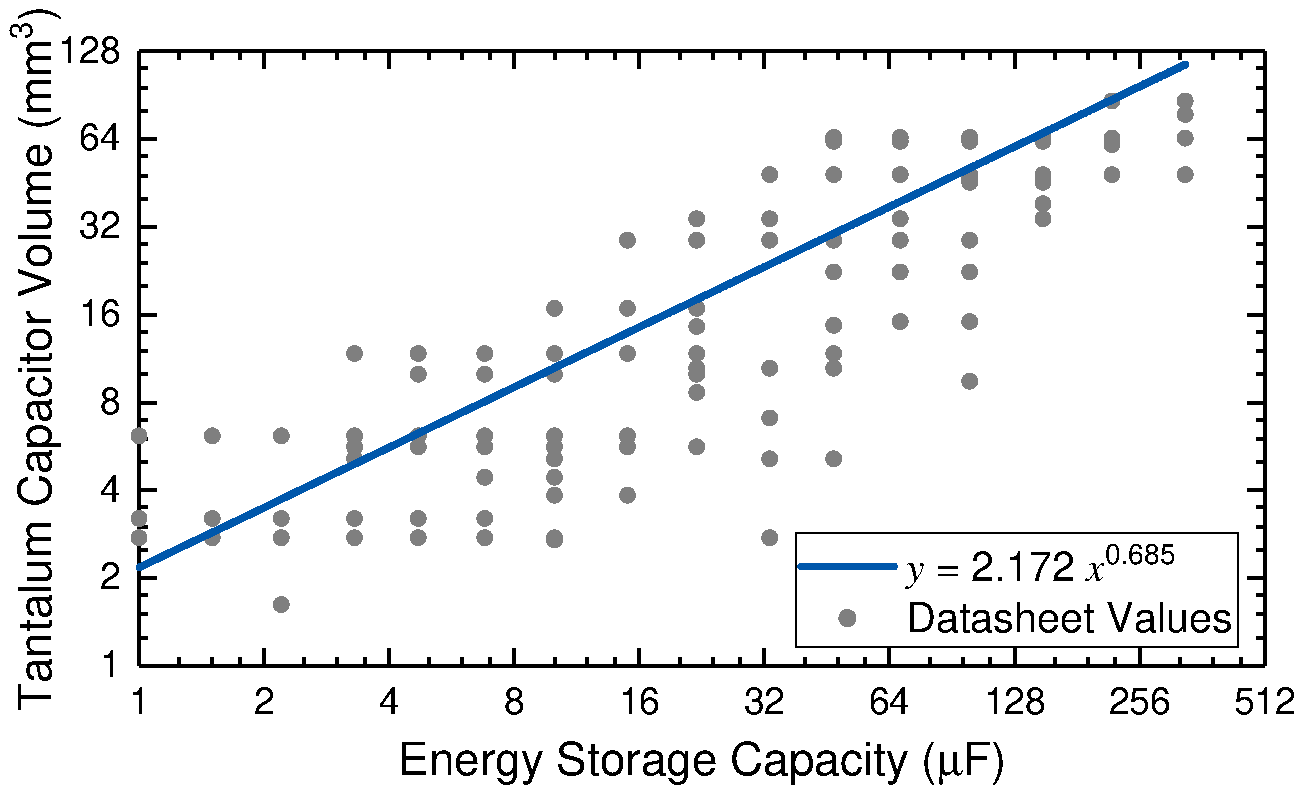
\includegraphics[width=\columnwidth]{ch4_sizingapproach/figures/CapVol2Fig2}
    \caption{Tantalum capacitor volume against capacitance for the six series of capacitors analysed. }
    \label{fig:capvol}
\end{figure}

\subsubsection{Metric of Interruption Periods} \label{subsubsec:metricintper}

% Definition/Measurement of interruption periods. recharging ability? Considering leakage?
% why interruption periods is important, why we consider it.

% , i.e. the period that does not make forward progress. The total interruption periods should be opposite to forward progress. 
Applications may have various requirements on interruption periods. 
To demonstrate the usage of our sizing approach, we consider a designer requests the 90th percentile of all interruption periods as an example metric of interruption periods, denoted as \nm{T}{int}. 
This metric indicates 90\% of interruption periods are shorter than \nm{T}{int}. 
This metric can be adapted for particular application requirements. 
% In We assume that $T_{interrupt}$ is preferable to be short for general application. 

\subsubsection{Cost Function}

From the previous observations (\fref{fig:maxfwp}) we can see that achieving the optimal progress improvement costs much more capacitance (mean 3.2$\times$) than to achieve 95\% improvement. 
A trade-off is necessary to improve forward progress while restricting the overheads of increased capacitor volume and interruption periods. 
This involves a problem of multi-criteria decision making~\cite{triantaphyllou2000multi}, which is outside the scope of this work. 
Nevertheless, we provide a cost function in (\ref{eq:tradeoff}) as an example to illustrate how these three factors could be traded-off, but designers are expected to customise a cost function with parameters of importance to specific application requirements. 
Note that the function (\ref{eq:tradeoff}) is to be maximised to find the recommended capacitance. 
\begin{equation}
    f = \frac{\nmm{\alpha}{exe}}{\nmm{k}{1}} - \left(\frac{\nmm{v}{cap}}{\nmm{k}{2}}\right) ^ {2} - \left(\frac{\nmm{T}{int}}{\nmm{k}{3}}\right) ^ {2} 
    \label{eq:tradeoff}
\end{equation}
\nm{\alpha}{exe} denotes normalised forward progress, \nm{v}{cap} denotes capacitor volume, and \nm{T}{int} denotes application interruption periods as mentioned in \sref{subsubsec:metricintper}. 
\nm{\alpha}{exe}, \nm{v}{cap}, and \nm{T}{int} can be generated from the simulation tool given $C$ as an input. 
\nm{k}{1}, \nm{k}{2}, and \nm{k}{3} are coefficients for normalising each metric, and they are empirically determined according to applications. 
In this example, the undesirable parameters are expressed as quadratic and negative terms to give an increasing cost to higher values. 
While only three parameters are considered here, others (such as the energy harvester size) could be included for a system-wise sizing scenario.
As an example to demonstrate its usage, we arbitrarily configure the function by setting \nm{k}{1} = 0.2, \nm{k}{2} = \SI{200}{\cubic\milli\meter}, and \nm{k}{3} = \SI{500}{\milli\second}. 
%, i.e.:
%\begin{equation}
%    f = \frac{\nmm{\alpha}{exe}}{0.2} - (\frac{\nmm{v}{cap}}{200}) ^ {2} - T_{recharge} ^ {2} 
%    \label{eq:tradeoffuse}
%\end{equation}
% where \nm{v}{cap} is in \SI{}{\cubic\milli\meter} and $T_{recharge}$ is in second. Here, $\frac{1}{\nmm{k}{1}} / \frac{1}{\nmm{k}{2}}$ equals 1000, but this does not mean that forward progress is 1000 times more important than capacitor volume.

\subsubsection{Results}

The effect of the trade-off is plotted in \fref{fig:tradeoff} using the Denver 2018 energy source dataset. 
Compared to the capacitor size that solely maximises forward progress, on average, an appropriately-sized capacitor achieves 93\% of the maximum forward progress, while saving 83\% of capacitor volume and 91\% of interruption periods. 
This also demonstrates the efficacy of the cost function and the chosen coefficients. 
Compared to the minimum storage case, the appropriately-sized capacitor improves forward progress by 12-124\% with energy storage increased from \SI{6.2}{\micro\farad} to \SI{30}{\micro\farad}.

\begin{figure}
    \centering
    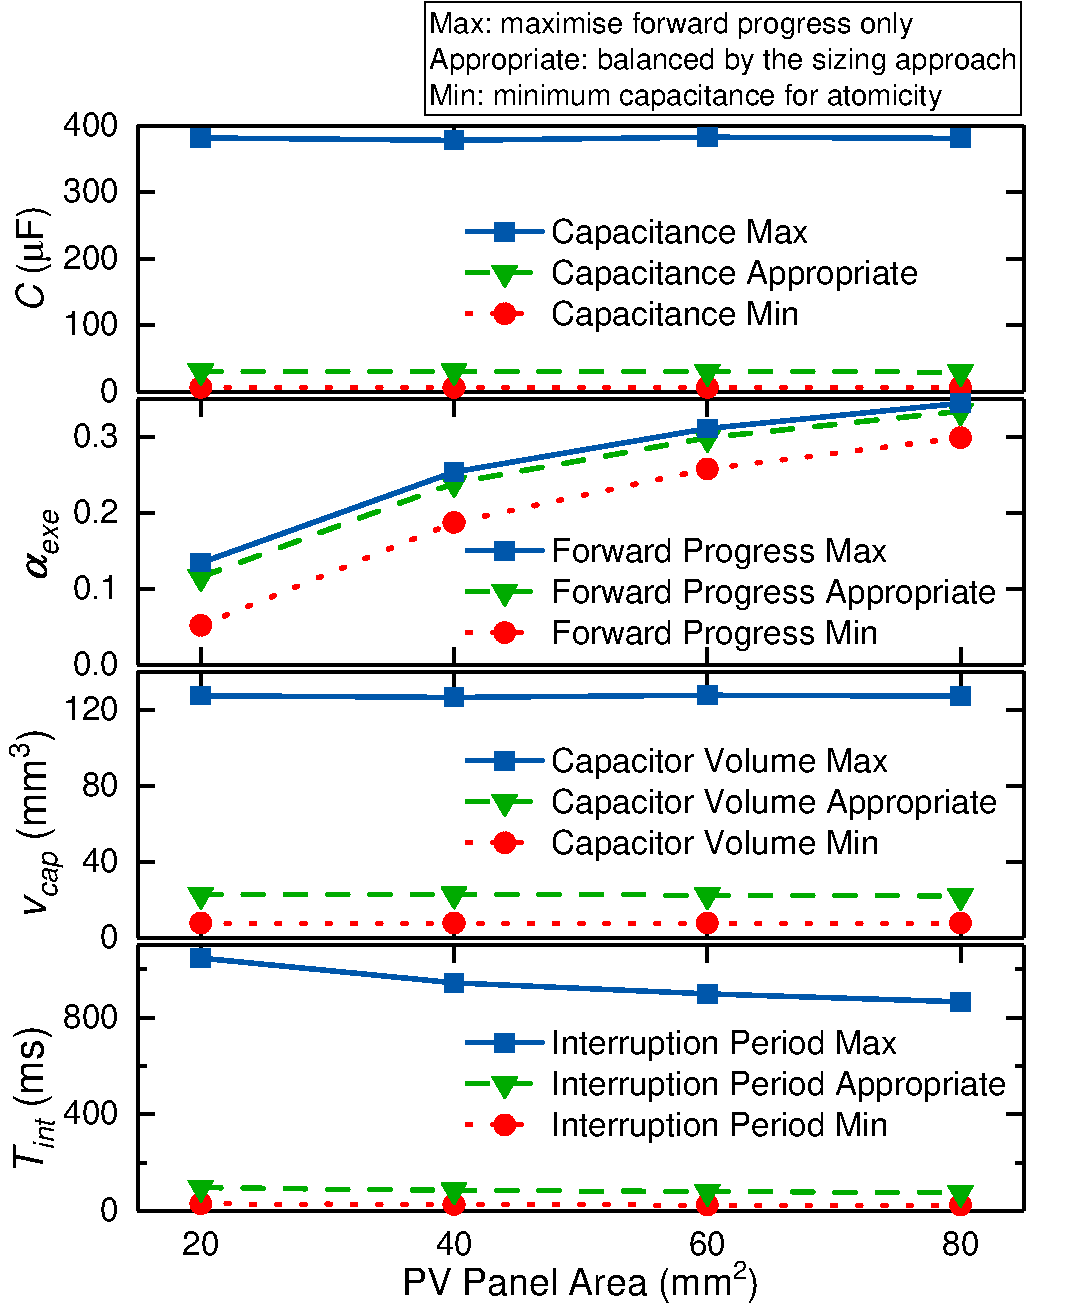
\includegraphics[width=\columnwidth]{ch4_sizingapproach/figures/Tradeoff3Fig}
    \caption{The sizing approach trades off forward progress, capacitor volume, and interruption periods. The results are plotted against a range of PV panel area, given Denver 2018 energy source dataset. }
    \label{fig:tradeoff}
\end{figure}

As shown in \fref{fig:capvol}, the closest available capacitance that satisfies the \SI{6.2}{\micro\farad} minimum capacitance is \SI{6.8}{\micro\farad}, whereas the closest available capacitance to the appropriate \SI{30}{\micro\farad} is \SI{33}{\micro\farad}. 
The minimum volumes of \SI{6.8}{\micro\farad} and \SI{33}{\micro\farad} capacitors are both \SI{2.75}{\cubic\milli\meter}, which means using the appropriate capacitance, instead of the minimum one, may not incur dimensional overhead. 
% For \SI{47}{\micro\farad}, the absolute volume (\SI{5.12}{\cubic\milli\meter}) is insignificant compared to the device as a whole, e.g. an MSP430FR6989 MCU chip alone occupies \SI{274.4}{\cubic\milli\meter} (14 $\times$ 14 $\times$ 1.4). 
The regressed volume of the above two capacitance values are \SI{8.1}{\cubic\milli\meter} and \SI{23.8}{\cubic\milli\meter} respectively. 
However, the selection of capacitors can be dependent on factors other than physical volume, such as reliability, operation temperature, and more specific application needs. 
These factors can also be added into the cost function if necessary. 
% Again, such a volume scale is still insignificant in a whole device. 

